%%PREAMBLE %%%%%%%%%%%%%%%%%%%%%%%%%%%%
\documentclass[10pt, a4paper]{article}% size of txt = 10pt
\usepackage[top= 2cm,
			bottom = 2cm,
			left = 1.7cm,
			right = 1.7cm,
			footskip = 0.5cm,
			headsep = 0cm,
			headheight = 0cm
					]{geometry}
\usepackage{amsmath} % math packages
\usepackage{amsfonts}% math packages
\usepackage{amssymb} % math packages
\usepackage{graphicx} %package for including graphics
\usepackage{array}
\usepackage[thinlines]{easytable}
\usepackage{float}
\usepackage[section]{placeins}
\usepackage[hidelinks]{hyperref}
\usepackage[shortlabels]{enumitem}
\usepackage{svg}
\usepackage{bigstrut}
\usepackage{wrapfig,lipsum,booktabs}
\usepackage{subcaption}
\usepackage{xfrac}
\usepackage{pdfpages}
\usepackage{listings}
\usepackage{xcolor}

\usepackage{listings}
\usepackage{color} %red, green, blue, yellow, cyan, magenta, black, white
\definecolor{mygreen}{RGB}{28,172,0} % color values Red, Green, Blue
\definecolor{mylilas}{RGB}{170,55,241}

\definecolor{codegreen}{rgb}{0,0.6,0}
\definecolor{codegray}{rgb}{0.5,0.5,0.5}
\definecolor{codepurple}{rgb}{0.58,0,0.82}
\definecolor{backcolour}{rgb}{1,1,1}

\lstdefinestyle{mystyle}{
    backgroundcolor=\color{backcolour},   
    commentstyle=\color{codegreen},
    keywordstyle=\color{magenta},
    numberstyle=\tiny\color{codegray},
    stringstyle=\color{codepurple},
    basicstyle=\ttfamily\footnotesize,
    breakatwhitespace=false,         
    breaklines=true,                 
    captionpos=b,                    
    keepspaces=true,                 
    numbers=left,                    
    numbersep=5pt,                  
    showspaces=false,                
    showstringspaces=false,
    showtabs=false,                  
    tabsize=2
}
\lstset{style=mystyle}


%date format
\def\mydate{\leavevmode\hbox{\twodigits\day.\twodigits\month.\the\year}}
\def\twodigits#1{\ifnum#1<10 0\fi\the#1}


\usepackage[T1]{fontenc} 
\usepackage{lmodern}
\usepackage{indentfirst}
\setlength{\parindent}{1cm}

\makeatletter
\newcommand{\thickhline}{%
    \noalign {\ifnum 0=`}\fi \hrule height 2pt
    \futurelet \reserved@a \@xhline
}
\newcolumntype{"}{@{\hskip\tabcolsep\vrule width 2pt\hskip\tabcolsep}}
\makeatother
\newcolumntype{?}{!{\vrule width 2pt}}
%%DOC ENVIROMENT%%%%%%%%%%%%%%%%%%%%%%%
\begin{document}
%Title 
\begin{flushleft}%% left justification
	\textbf{\Large{MKC-KBC: Úkol č. 6}}\hfill Filip Paul\\
	\large{Patch anténa v blízkosti lidských tkání \hfill\mydate}
\end{flushleft}

\section{\Large 3D modely zkoumaných scénářů:}
\begin{figure}[ht!]
	\centering
	\begin{minipage}{0.32\textwidth}
		\centering
		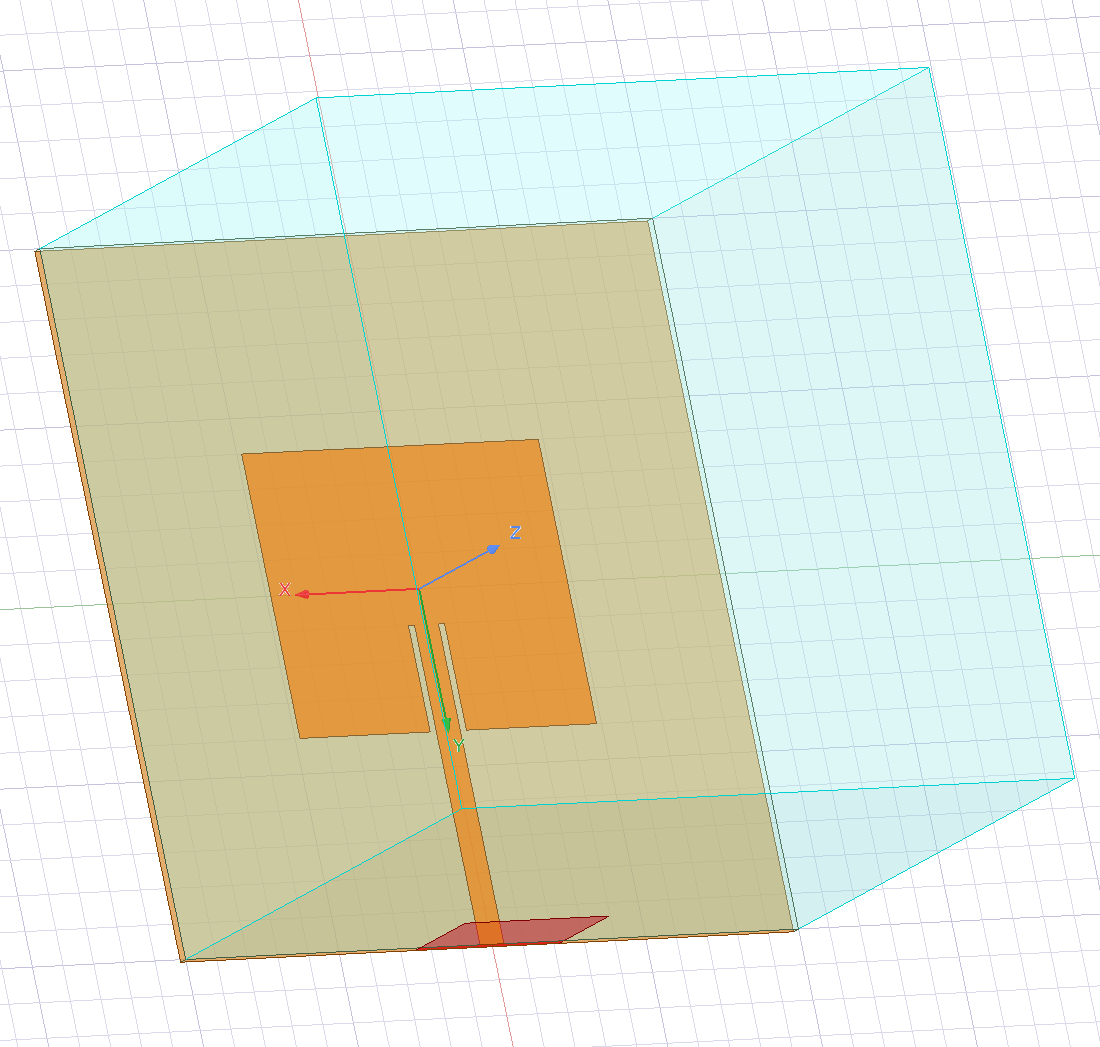
\includegraphics[width= 1\textwidth, height = 0.25\textheight]{3D_model_free_space.png}
		\captionof{figure}{3D - Free space - direct feed}
	\end{minipage}%
	\hfill
	\begin{minipage}{0.32\textwidth}
		\centering
		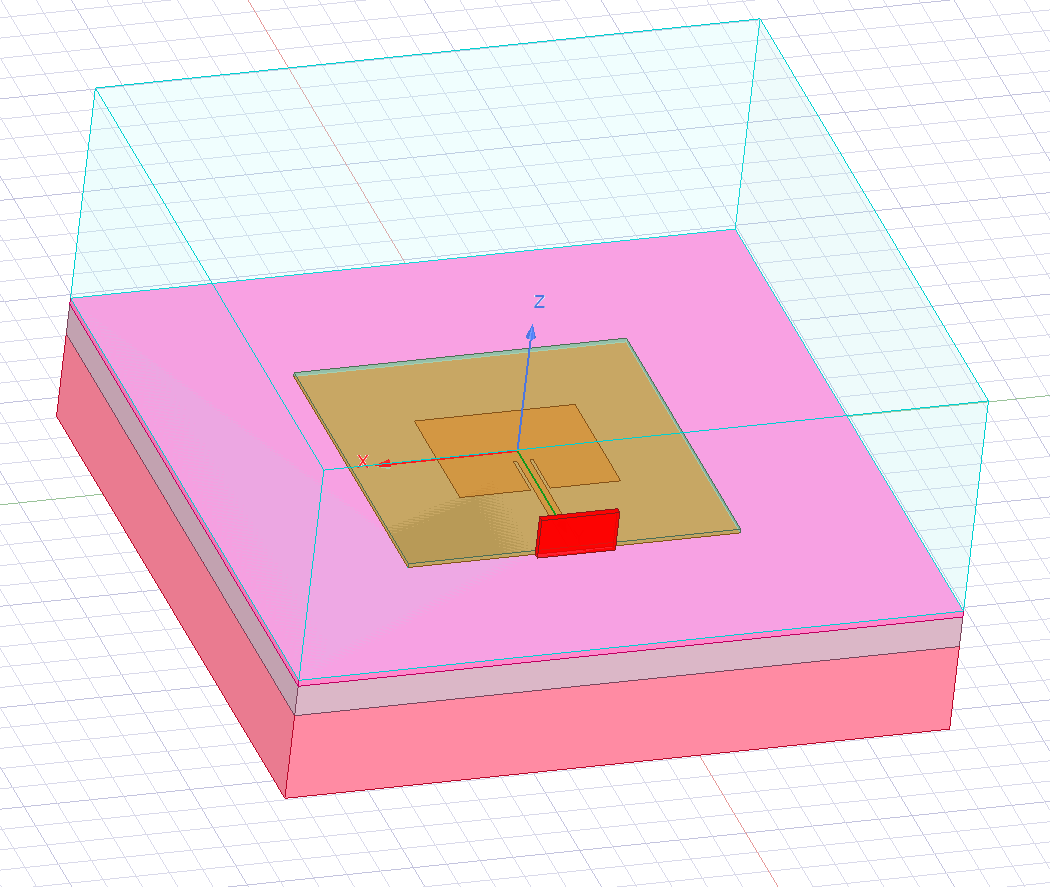
\includegraphics[width= 1\textwidth,height = 0.25\textheight]{3D_model.png}
		\captionof{figure}{3D - phantom - direct feed}
	\end{minipage}
	\hfill
	\begin{minipage}{0.32\textwidth}
		\centering
		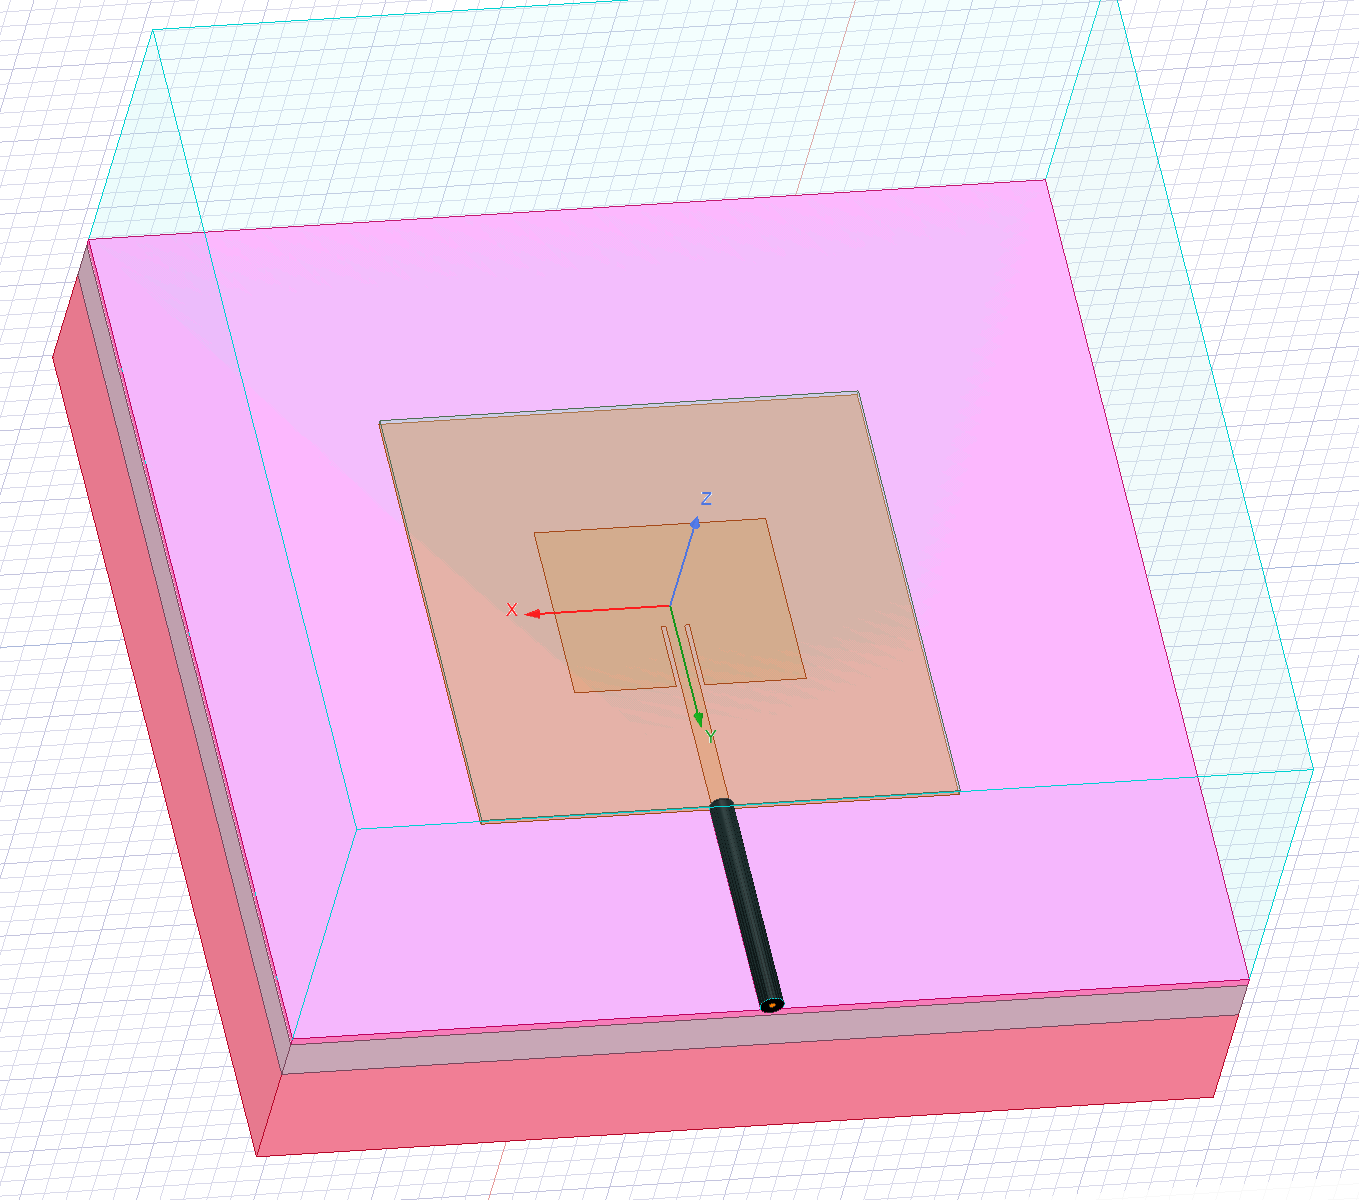
\includegraphics[width= 1\textwidth,height = 0.25\textheight]{3D_model_koax.png}
		\captionof{figure}{3D - phantom - coaxial feed}
	\end{minipage}
	\end{figure}

\section{\Large Porovnání S11 parametrů:}
Z níže přiloženého grafu parametrů S11 pro různé scénáře je patrné, že se 
rezonanční frekvence patch antény mírně snížila v případě použití antény
poblíž lidských tkání.
\begin{figure}[ht!]	
\centering
		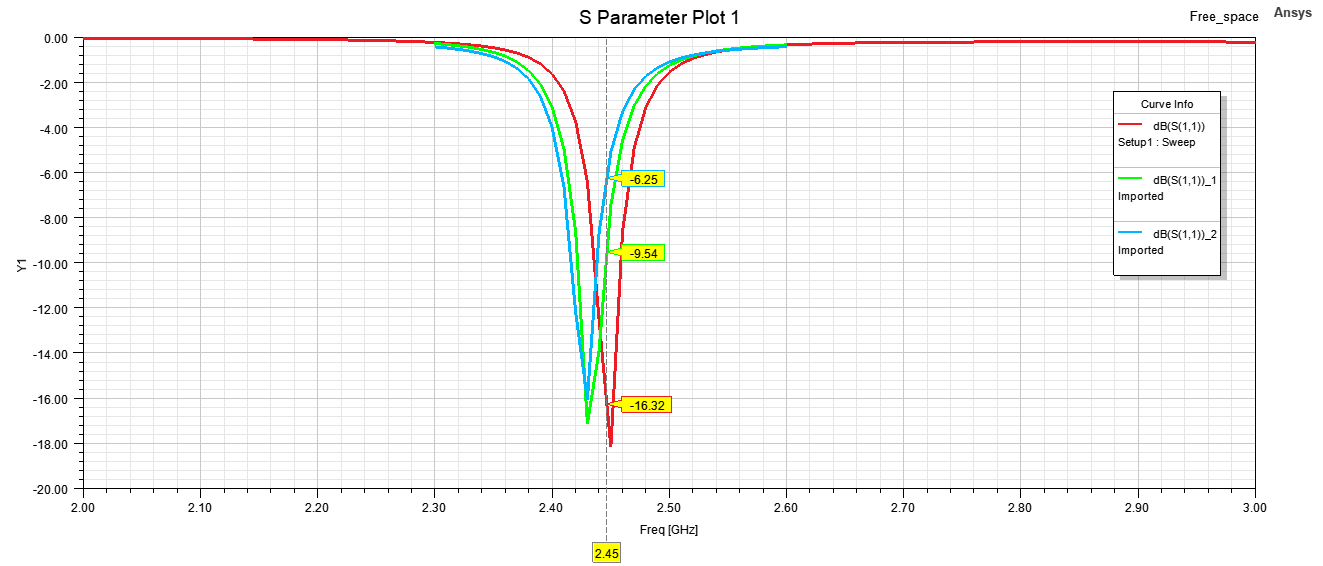
\includegraphics[height = 0.3\textheight]{S11_free_space.png}
		\captionof{figure}{Porovnání S11 parametrů pro jednotlivé scénáře (Free space - červeně,
		Phantom direct feed - zeleně a Phantom coaxial feed - modře)}
\end{figure}
\clearpage

\section{\Large Porovnání charakteristické impedance portu (místa buzení):}
Přiložení patch antény k lidským tkáním má pouze nepatrný vliv na impedanční přizpůsobení,
to je pravděpodobně způsobeno tím, že patch anténa má reflektor, který do jisté míry odstraňuje
vliv okolního prostředí (ve směru pod reflektorem).
\begin{figure}[ht!]	
\centering
		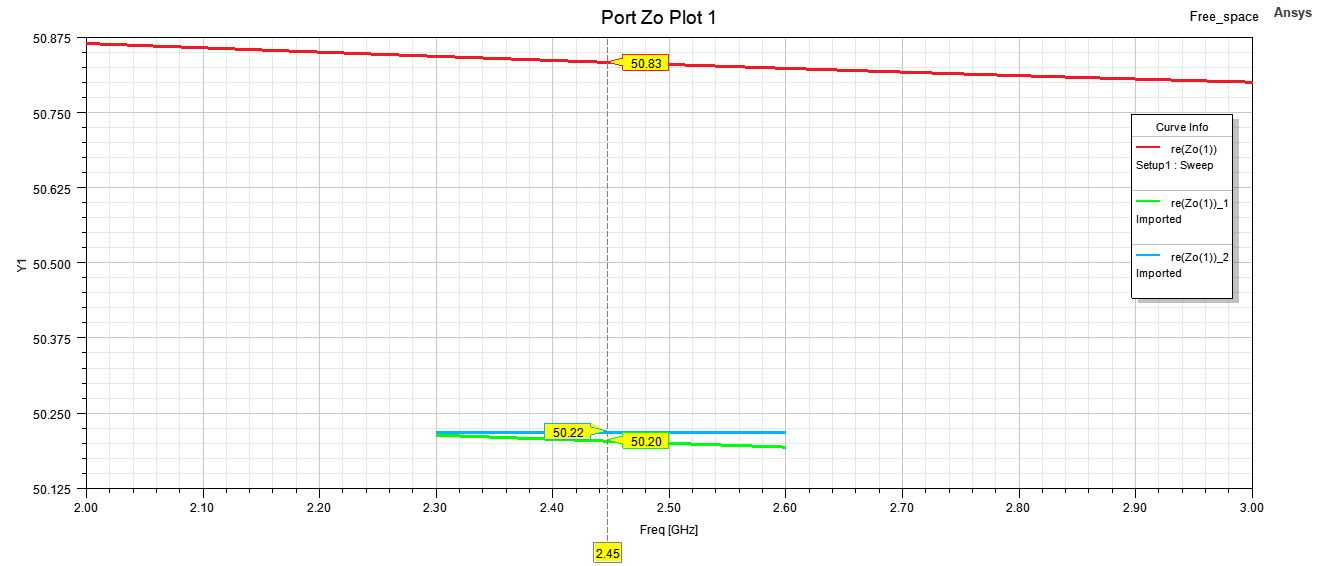
\includegraphics[height = 0.3\textheight]{Z0_free_space.png}
		\captionof{figure}{Porovnání Z0 pro jednotlivé scénáře (Free space - červeně,
		Phantom direct feed - zeleně a Phantom coaxial feed - modře)}
\end{figure}

\section{\Large Porovnání vyzařovacích charakteristik:}
Následující grafy zobrazují vyzařovací charakteristiky v dB a lineárních 
jednotkách. V případě umístění antény do blízkosti lidských tkání dojde k určité deformaci
vyzařovací charakteristiky. Deformace však není úplně výrazná. Zároveň se možná v simulaci objevují
rozdíly způsobené zvětšením "objemu" radiačních podmínek.
Při simulaci došlo k mírnému zvýšení maximálního zisku z 7.5 dB na 8 dB.

\begin{figure}[ht!]
	\centering
	\begin{minipage}{0.32\textwidth}
		\centering
		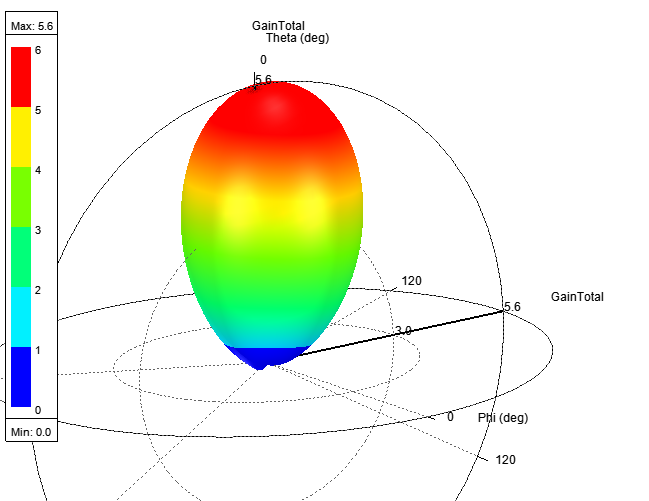
\includegraphics[width= 1\textwidth]{RAD_LIN_free_space.png}
		\captionof{figure}{Free space - gain[-]}
	\end{minipage}%
	\hfill
	\begin{minipage}{0.32\textwidth}
		\centering
		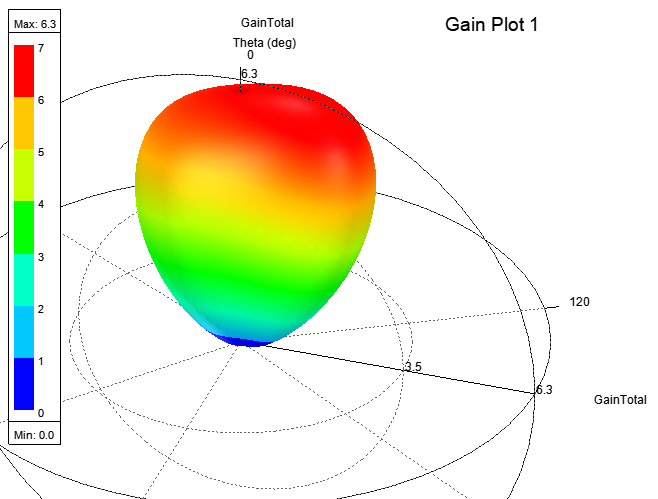
\includegraphics[width= 1\textwidth]{RAD_lin_phantom.png}
		\captionof{figure}{phantom direct feed - gain[-]}
	\end{minipage}
	\hfill
	\begin{minipage}{0.32\textwidth}
		\centering
		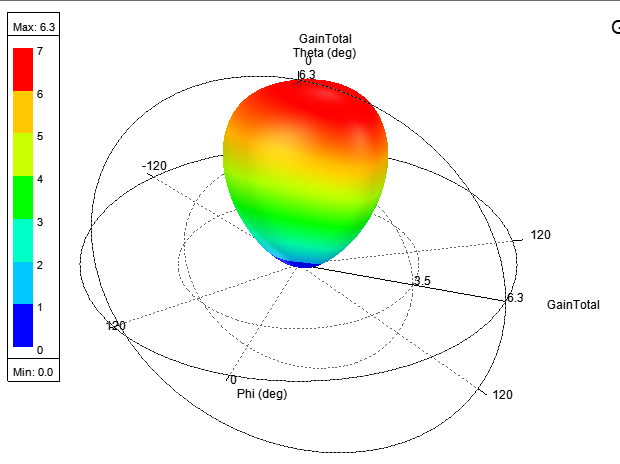
\includegraphics[width= 1\textwidth]{RAD_lin_coax.png}
		\captionof{figure}{phantom coaxial feed - gain[-]}
	\end{minipage}
	\end{figure}
\clearpage
\begin{figure}[ht!]
	\centering
	\begin{minipage}{0.32\textwidth}
		\centering
		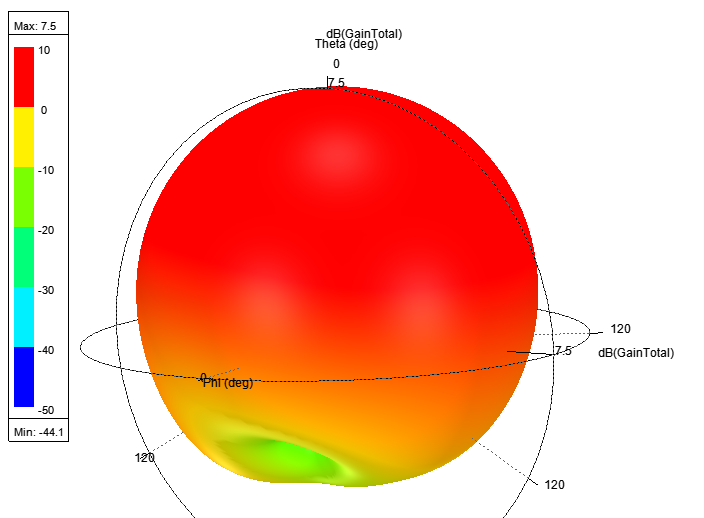
\includegraphics[width= 1\textwidth]{RAD_dB_free_space.png}
		\captionof{figure}{Free space - gain[dB]}
	\end{minipage}%
	\hfill
	\begin{minipage}{0.32\textwidth}
		\centering
		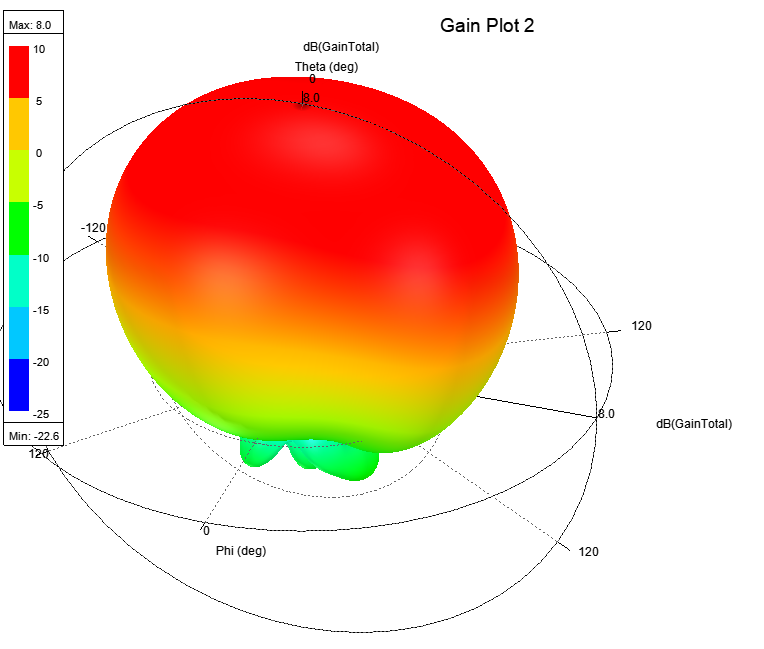
\includegraphics[width= 1\textwidth]{RAD_dB_phantom.png}
		\captionof{figure}{phantom direct feed - gain[dB]}
	\end{minipage}
	\hfill
	\begin{minipage}{0.32\textwidth}
		\centering
		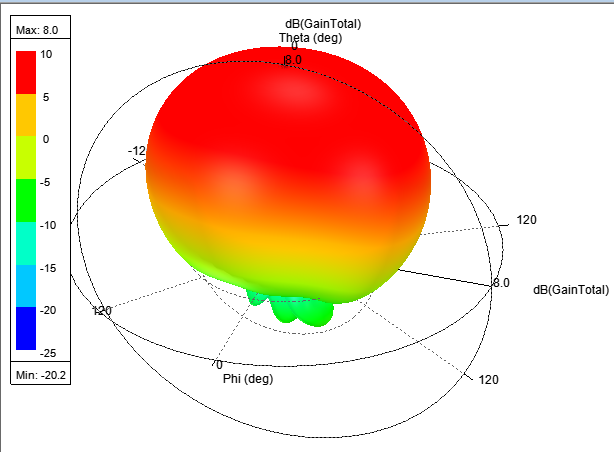
\includegraphics[width= 1\textwidth]{RAD_dB_coax.png}
		\captionof{figure}{phantom coaxial feed - gain[dB]}
	\end{minipage}


	\end{figure}

	\section{\Large Rozložení E pole}
	Rozložení pole E je téměř identické pro všechny 3 scénáře. Na obr. 13
	sice vypadá rozložení rozdílně, to je však způsobeno fázovým posunem,
	který přidává nenulová délka koaxiálního kabelu. V případě zobrazení pole
	E v případě scénáře s koaxiálním kabelem s nenulovou fází (obr 15 pro fázi 110$\deg$)
	dostáváme podobné rozložení pole jako u předhozích scénářů.
\begin{figure}[ht!]
	\centering
	\begin{minipage}{0.32\textwidth}
		\centering
		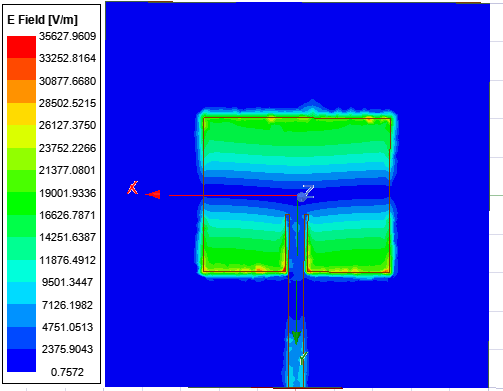
\includegraphics[width= 1\textwidth]{EFIELD_free_space.png}
		\captionof{figure}{Free space - E field}
	\end{minipage}%
	\hfill
	\begin{minipage}{0.32\textwidth}
		\centering
		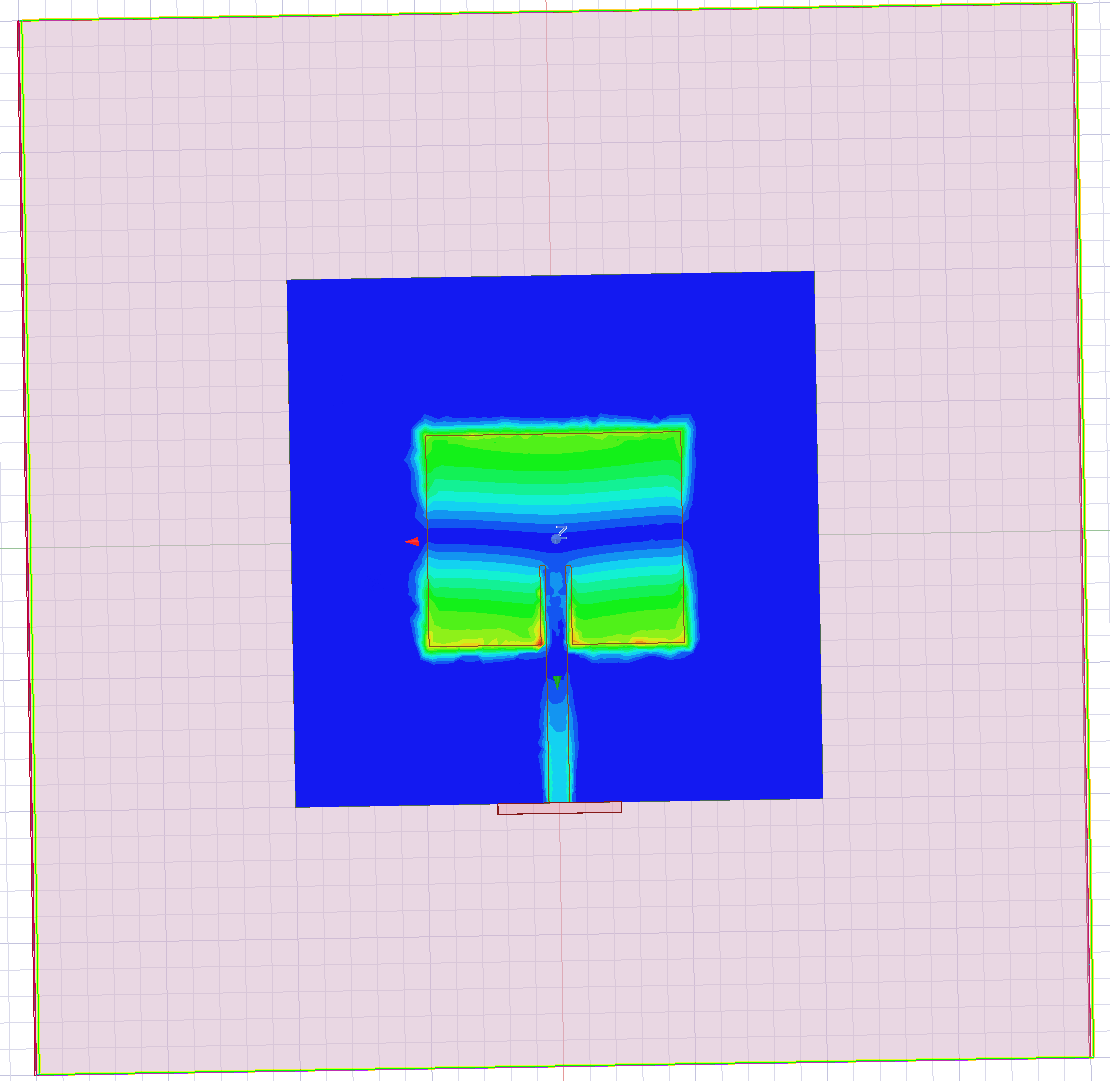
\includegraphics[width= 1\textwidth]{EFIELD_phantom.png}
		\captionof{figure}{phantom direct feed - E field}
	\end{minipage}
	\hfill
	\begin{minipage}{0.32\textwidth}
		\centering
		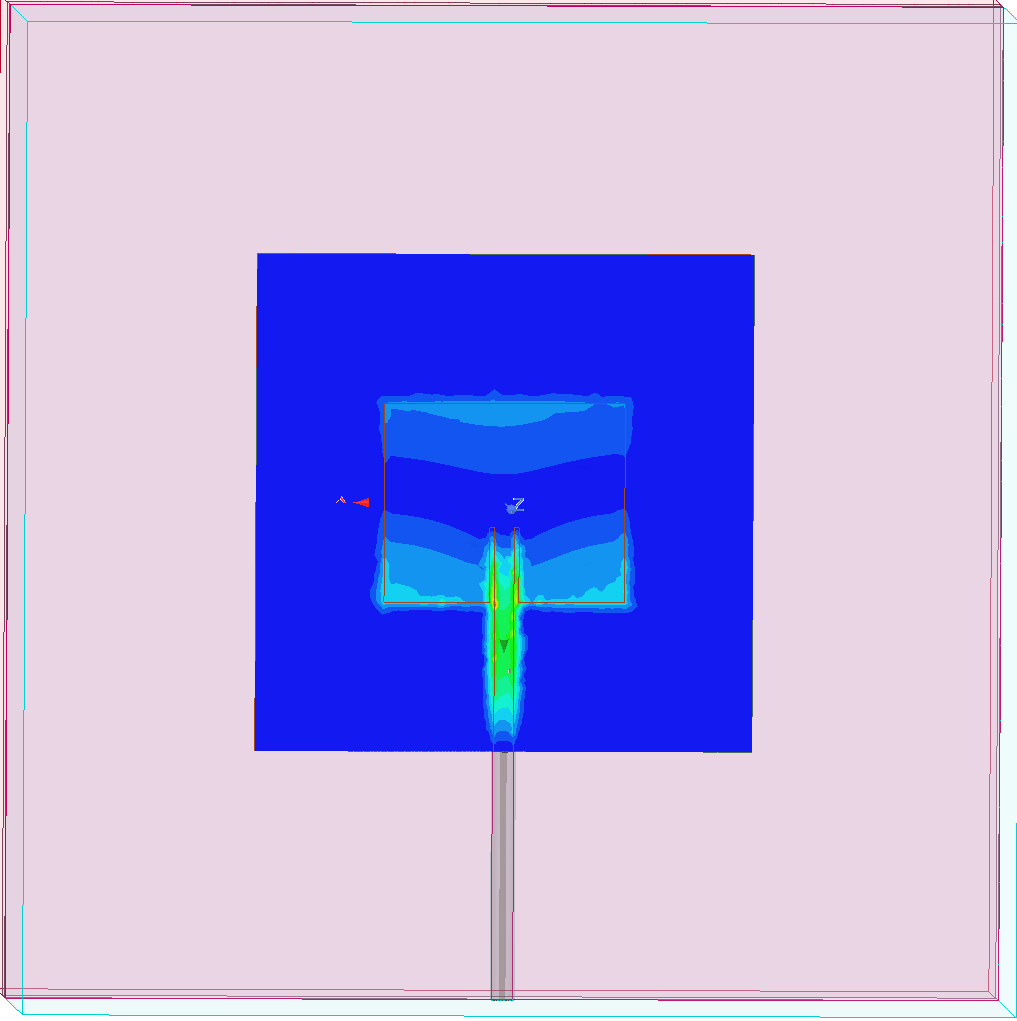
\includegraphics[width= 1\textwidth]{EFIELD_coax.png}
		\captionof{figure}{phantom coaxial feed - E field}
	\end{minipage}
	\end{figure}

\begin{figure}[ht!]
\centering
	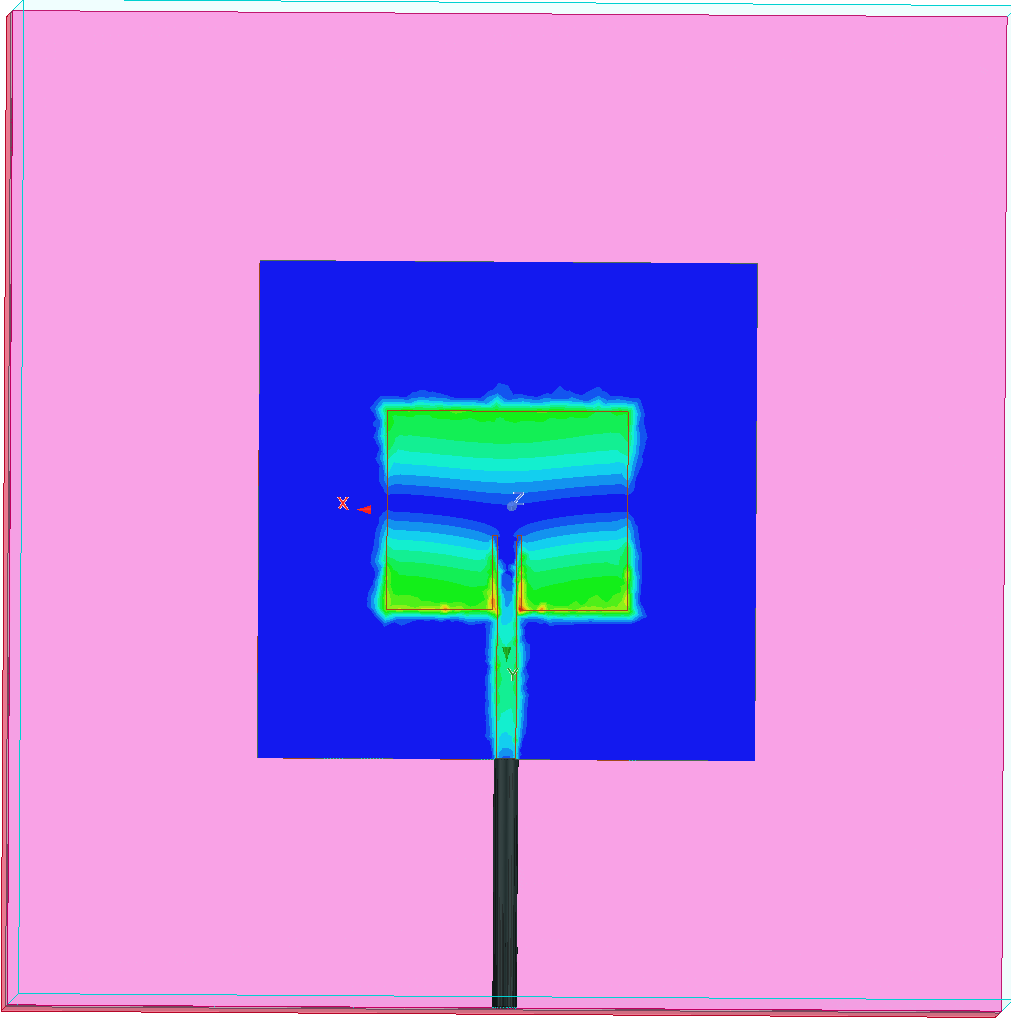
\includegraphics[height = 0.25\textheight]{EFIELD_coax_phase.png}
	\captionof{figure}{E field - phase 110$\deg$}
\end{figure}
\clearpage
\begin{figure}[ht!]
	\centering
		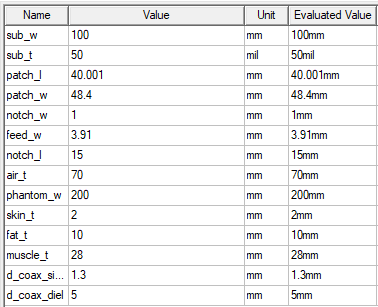
\includegraphics[]{variables.png}
		\captionof{figure}{Parametry simulace}
	\end{figure}



\end{document}

%\[f(x)= (x+2)^2 - \frac{9\cdot 2\pi}{26}\] %%mathematic equatation in display style mode
%%optional:
%	\begin{align} %%this alignes all charakters after & if *is removed equations will be numbered
%	\hspace{5cm}  
%		 x &= a_2 x^2 +_1 x + a_0 \\
% 		x &=x^2 \nonumber		%no number will not add number to eq
%	\end{align}
